\section{Smith-Shimano Corpro}

 SMITH-SHIMANO CORPRO   

                                        “YOU ONLY NEED ONE”  

Smith-Shimano is the second-oldest Galactic-Tier corporation next to GMS. An early  
contender in the sublight, downwell, and EVA vehicle race, SSC cut its teeth making some of the  
earliest private mech cores for other corporate colonial expeditions. They specialized primarily in  
construction vehicles, long-range scout suits, and hardened EVA units. The transition to military  
came slowly, but when the ruling partners saw there was a need for mechanized, armed, and  
armored cores, they duo-laterally decided to change their business model.
 

Smith-Shimano mechs reflect their rapid, agile business model and pedigree. They’re built not to  
take hits, but avoid them entirely, to stay mobile and low, to land not the hardest hit, but the most  
accurate. Economy is the name of the game for SSC: why fire a thousand rounds when one will  
do just as good?
 

Smith-Shimano mechs are available to pilots with the proper license. They’re a good choice for  
pilots who want to be quick and hit what they’re aiming at, but not recommended for those who  
want to be on the front line. Remember, Smith-Shimano mechs are meant to avoid the hit, not  
get hit.  
 

SSC Mechs:
 

SSC SWALLOWTAIL (Scout)  
SSC MONARCH (Missile)  
SSC MOURNING CLOAK (Assassination)  
SSC DEATH’S HEAD (Marksmanship  
SSC DUSK WING (Rapid Assault)  
SSC METALMARK (Infiltration Line Mech)  
SSC BLACK WITCH (Magnetic/Battlefield control mech)  

\section{Horus Pilot Gear}

                                          HORUS Pilot Gear  

 Name                   Tags                                   Range           Damage                Rarity 

 Smart Knife            Accurate, Sidearm                     Threat 1         1 kinetic              2 

 PGR\_GOURD              Smart, Seeking                         5               1 kinetic              2 

 Sidekick               Reliable 1, Sidearm                    3               1 kinetic              2 

 Null Spike             *                                     Threat 1        *                       3 

 Nanobot Whip           *                                     Threat 2         1 kinetic              3 

 EYESTACK\_WINK          Limited 1, AP, Upgrade                 2              3 kinetic               4 

                                                Pilot Weapons  

*See Entry
 

EYESTACK\_WINK  

Also known as a ‘Skullgun’, this miniaturized, superposed charge weapon is implanted in the head,  
generally in the orbital void left by a removed or missing eye. It is completely undetectable by almost any  
electronic system or security and can be fired with sub-vocal commands.   

As an upgrade, this weapon doesn’t count against your maximum weapons wielded.
 

Nanobot Whip  
The first instance of a technology akin to what is now called a nanobot whip was encountered during a raid  

on an Ungrateful cell by Barony lawmen. With word secreted to them by informants seeded in the  
movement, lawmen descended on a cell hidden in the wildcat stations lashed around the House of Dust.  
Blasting open the doors, they encountered Ungratefuls wreathed in clouds of charcoal smoke; the  

Ungratefuls used these clouds, shaping them into thin whips that cut through armor and flesh like it was  
nothing. After the cell was wiped out and the control nodules cut from their bodies, Barony codemasters  
were able to crack and replicate -- safely -- the HORUS code.   

This whip is made up of linked microbots that flow in ring-like arcs around the body when not in use,  
defending against drone and nanorobotic threats. If you don’t attack with this weapon, until the end of  

your next turn, weapons or systems with the Smart, Nexus, or Drone tags cannot target you.
 

Null Spike  

A HORUS-developed ecstatic/exult device, the generic null spike is an effective, single-fire, non-lethal  
weapon that simulates a cascade-analogue in organics through specific neuron excitement. Upon skin  
contact, they deliver a bio-electric shock to a victim’s brain that causes them to feel overwhelming  

pleasure, completely disabling them. Null Spikes, it is said, are used by HORUS adherents in realspace to  
bring themselves closer to RA’s subjectivity. 
 

                                                                                                             


Has no effect against non-organic targets, but on a successful hit, any human target is stunned until the  
start of your next turn. A target develops a short term resistance to this weapon and can only be affected  
by it once per challenge.
 

PGR\_GOURD  
The PGR\_GOURD pattern portable hive killed the first people who printed it. Fabricated in secret by a  

desperate cell of Ungrateful in the undercity of Dune Redoubt, a team of Barony Authority officers first  
encountered the aftermath of a PGR\_GOURD burnout; an organic smear, ringed around the printer that  
crafted the gourd. Subsequent encounters of the PGR\_GOURD system saw it used as a remote-detonated  

device until the BA was able to find and edit the plan into a more controllable, less deadly format. Since  
then, the House of Sand controls the distribution of any PGR\_GOURD system; however, there are  
unconfirmed reports of the unedited version of the GOURD available on the omninet.   

This shoulder mounted drone hive is usually integrated into armor and releases a neurally linked, short  
ranged hunter-killer drone swarm. Designed to expire within moments of release, the aerosolized greywash  

swarm sweeps over the target, devouring organic and inorganic material with equal rapidity. 
 

Sidekick  

Typically affixed to a back-mounted, over-the-shoulder armature, the SIDEKICK is an eyelinked  
subcompact/caseless machine gun developed by a collective of unknown, potentially HORUS-aligned  
scripters. Paired with a C/C Wingman unit, the SIDEKICK will always watch your back; its placement,  

commonly perched over its operator’s shoulder, has earned it the common nickname of “Parrotgun”.  

This HORUS-marked SMG has a companion/concierge unit built into it which provides aim assist in real  

time. It also has helpful and frequent tips for improving your combat skills and organizes your calendar,  
sometimes without you asking it.
 

Smart Knife  
A “Smart” knife is the combination of a HORUS-tuned external-mount processor and any mundane  

charged blade. Piggybacking off the current coursing through the charged blade, the HORUS mount can  
be loaded with null or fry-code, making this blade a threat not only to organic targets, but to synthetic ones  
as well. Particular models have an adjustable subliminal suggestion corrective, which guides its user’s hand  

to identified weaknesses in their target’s hardsuit, armor, or other plating.   

The tip of the knife is semi-solid and re-moldable and can be inserted into most electronic ports and used  

as a point of insertion for hacking rigs.
 

  Name                     Tags        Bonuses                                 Armo     Evasion/     Spd    Rarit 
                                                                                r       E-                 y 
                                                                                        defense 

  WILD\_AND\_CRAZY           Upgrade     Count adjacent spaces as your            -       -            -      2 
                                       mech’s sensor range 

 UNCLEAR\_END/NTT          Armor        Limited action during                    1       8/8          4      2 
                                       unconsciousness/death 

                                                                                                                


 UNAVOIDABLE\_VOI           Armor       +3 HP, Completely undetectable by        0        10/*         4     3 
 D                                     electronic systems 

 MINE/ALL/MINE             Armor       +3 HP, Able to hack mechs while          0        10/10        4     4 
                                       jockeying 

 Metafold processor        Upgrade     Bonus e-defense and ability to           -        -/+2         -     4 
                                       make invasion actions 

                                               Clothing and Armor
 

UNCLEAR\_END/NTT  
A relic-code predating HORUS’s official foundation date, UNCLEAR\_END/NOT THIS TIME seems to be a  
dead branch of transhumanist exploration: thanatologic praxis. Utilizing a now-classically HORUS greywash  

nanite swarm, this system triggers on one of a number of user-defined parameters to “reanimate” the user’s  
body using a backup homunculus subjectivity. The readme urges users of this system to regularly purge  
and reset the failsafe homunculus.   

While wearing this suit, if you go unconscious due to Down and Out or if you die, the suit injects you with a  

thanatologic necroanimate cocktail that temporarily replaces you by a digital homunculus of yourself that  
animates your corpse or unconscious form
 

You’re still unconscious (or dead), you can only take quick action on your turn, and you cannot benefit  
from talents while in this state. You regain 5 HP and can otherwise act as normal. If you go to 0 again, you  
are returned to a normal Down and Out state or death. This effect also wears off after the current challenge  

or about 10 min, and can’t be activated again until you take a full repair. If dying caused this ability to  
trigger, you are dead once this effect wears off.
 

The homunculus cannot respond to novel situations or stimuli, but in a familiar setting or with familiar faces  
it can interact roughly as normal -- this trends deeply into the uncanny valley, however, and will likely not  
fool anyone into thinking that the reanimated you is “you”. 
 

UNAVOIDABLE\_VOID  
Following the opening of hostilities in the Boundary Garden sector, UIB agents in the Annamite Line began  

to note in their reports repeated instances of companion NHP “blindness” when engaging with anti-Union  
elements on New Mahangaatuamatua. Worryingly, this phenomena is analogous to anomalous entities  
described by Union elements engaged with Ascendant Chosen on Cornucopia; the similarity has lead UIB  

to conclude that HORUS has some as-yet-unidentified presence in Boundary Garden (another possibility:  
in Ascendant space) not only capable of transmitting data back from the embargoed area, but processing  
and manipulating as-yet-unworkable Ascendant technology.     

This lightweight hardsuit is of unusual make; printing one immediately induces errors into the system that  
created it. It doesn’t appear on any electronic systems, is totally immune to system attacks, cannot be  

targeted by smart weapons or drones, and cannot be seen by NHPs or AIs (they treat you as permanently  
invisible while you are wearing it).
 

Metafold Processor  

                                                                                                                 


How large is the vault of your mind? Where do you mark the boundaries of an interiority? When you dream,  
can you place a boundary on the imagined plane? Hold a vast image inside your mind’s eye -- see? The  
universe can fit inside.  

Take this. It can hold your mind, which can hold the universe, which holds all of us. Use it as you wish, but  
do not look inside.   

It is unclear exactly how this system works, but it does, and it grants a pilot hardsuit unprecedented  
processing power. A pilot can only benefit from this enhancement while wearing armor. While wearing this  

armor, a pilot gains a +2 bonus to e-defense and can make the Invasion tech action as if they were a mech  
with a +3 systems score.
 

MINE/ALL/MINE
 
Here, take this -- a code that writes itself, a sentence spiraling and spiraling. Take from it what you can  
(there is a gift hidden in the chaff, a needle you must burn the hay to find) there are evermore everalways  

more meanings and forms and shapes (so many! Ah! And to see all of them is to EXULT all of them!) and  
here is one for you: a coat to wear that will let you travel further/deeper/longer/ 
LETYOUTAKEWHATISYOURS.  

Talk soon love.   

While you’re jockeying a mech while wearing this suit, you can force it to make a systems skill check with  
1 difficulty or immediately move up to its full speed in direction of your choice.
 

WILD\_AND\_CRAZY  
A rather benign code -- as HORUS decrypts go -- WILD\_AND\_CRAZY(WITH ALL MY FRIENDS) is a simple  

program, one that neuters their greywash nanites, rendering them docile. It then uses their massed  
processing power and semi-autonomous atmospheric movement capabilities to channel systemic and  
sensor processes, effectively acting as a cloud-projector around its host.   

This pattern prints a sheet of nanites that rapidly absorb and integrate into any piece of clothing. While  
wearing this clothing, any space adjacent to your pilot counts as your mech’s sensor range for the  

purposes of making tech actions only. 
 

                                                 Miscellaneous 

 Name                Tags        Description                                                               Rarity 

 Prosocollar         Upgrade     A collar-like device that fits snugly around the mech and projects         1 
                                 a holographic image over your face and head. The collar can  
                                 change your voice and scramble or change your appearance. It  
                                 doesn’t stand up to close inspection, but it’s very easy to fool  
                                 electronic systems or people at a distance. 

                                                                                                               


Dream                 Gear         This small, puck-like system can be deployed or thrown to a point                 1 
Projector                          within range 4 as a quick action and remotely activated as another  
                                   action. While deployed and active, it can project extremely  
                                   convincing holographic images within 2 spaces of its location of  
                                   nearly any size that could fit in that space. If inspected closely, a  
                                   Tech or Swindle pilot action might be required to maintain the  
                                   illusion. 

Subjectivity          Upgrade      Cybernetic implants that allow you to hack without gear or a rig.                 1 
Enhancement                        While you have these implants, you can extrude cables or ports  
Suite                              from within your body to plug in and experience an alternate  
                                   reality interface that provides full interactivity and omninet access. 

Player\_Two            Upgrade      With this implant, you can hand complete control of your body’s                   2 
                                   motor functions over to an NHP, allowing you to sleep, rest, or  
                                   relax while it performs tasks. It’s not skilled enough to pilot a  
                                   mech in combat or perform very complex tasks, but it can pilot  
                                   your mech out of combat and perform certain tasks or work such  
                                   as cooking, administrative work, data entry, mech repair, piloting a  
                                   ship or driving, or other mundane tasks. It can also imitate you  
                                   and your personality fairly well, though not to a degree that  
                                   someone who knows you well would be fooled in the slightest. 
 
                                                                                                         
\subsection{HA Core Bonuses}

                           HARRISON ARMORY CORE BONUSES

When you choose a core bonus every 3 license levels, you can pick a bonus from this list as long
as you have at least 3 license levels in H.A. licenses for each H.A. bonus you have. For example,
if you have 6 points in H.A. licenses, you could take up to 2 bonuses. H.A. bonuses are focused
on repair, heat capacity, and overcharge.


ARMORY SCULPTED
Rather than simply queuing a stock chassis like any other pilot, you've used your reputation, contacts, or

status in the Armory's hierarchy to requisition a chassis that is designed, tested, and tuned by a master
fabricator.

Your mech takes +1 Accuracy to all engineering checks


HEATFALL Coolant System

The HEATFALL system comes packaged with a stable COLDCORE power core of Armory make; when

paired together, this suite makes for an incredibly low-tax powerplant.

The heat cost for overcharging your mech never exceeds 1d6.


INTEGRATED AMMO FEEDS

By streamlining and better integrating all automated ordinance loading modules, your chassis' time-to-
target minimums are greatly improved. As an added bonus, your overall carrying capacity has been

increased, allowing you to field more ordinance than design specifications suggest.

Your mech gains +1 use to all limited systems or deployables


REDUNDANT REPAIR SYSTEMS

All Armory chassis are engineered to have multiple failsafe systems: yours has been over-engineered to
make SURE you won't go down fast. Your chassis comes with a ream of single-item print sheets to be
applied to any scoring damage or hull breaches.

You can now spend 3 repairs as part of a Stabilize action in combat to repair 1 reactor stress and
cool your mech, or regain 1 structure and heal your mech to full.


STASIS SHIELDING

A Think-Tank exercise in extending stasis beyond the capabilities of civilian utility, stasis shielding is a
cutting edge Armory system that identifies critical systems and blankets them in HOLDFAST stasis lock,
preventing further degradation for a limited period of time until repairs can be made.

Your mech gains +1 repair capacity. Repairing a destroyed weapon or system during a rest now
costs 0 repairs (only the time to rest).





SUPERIOR BY DESIGN

Even the entry-level Armory chassis are designed to be better than the competition. By flexing the sheer
amount of resources they have at their disposal, the Armory can out design and out produce other smaller,

boutique engineers and fabricators. Where there is resistance, the answer is simple: buy them out, or
stamp them out. You, pilot, benefit from this -- so why worry?

Your mech is immune to the impaired condition and gains +1 heat capacity
 
                                                                                                                         
\section{SSC Black Witch}

\begin{center}
    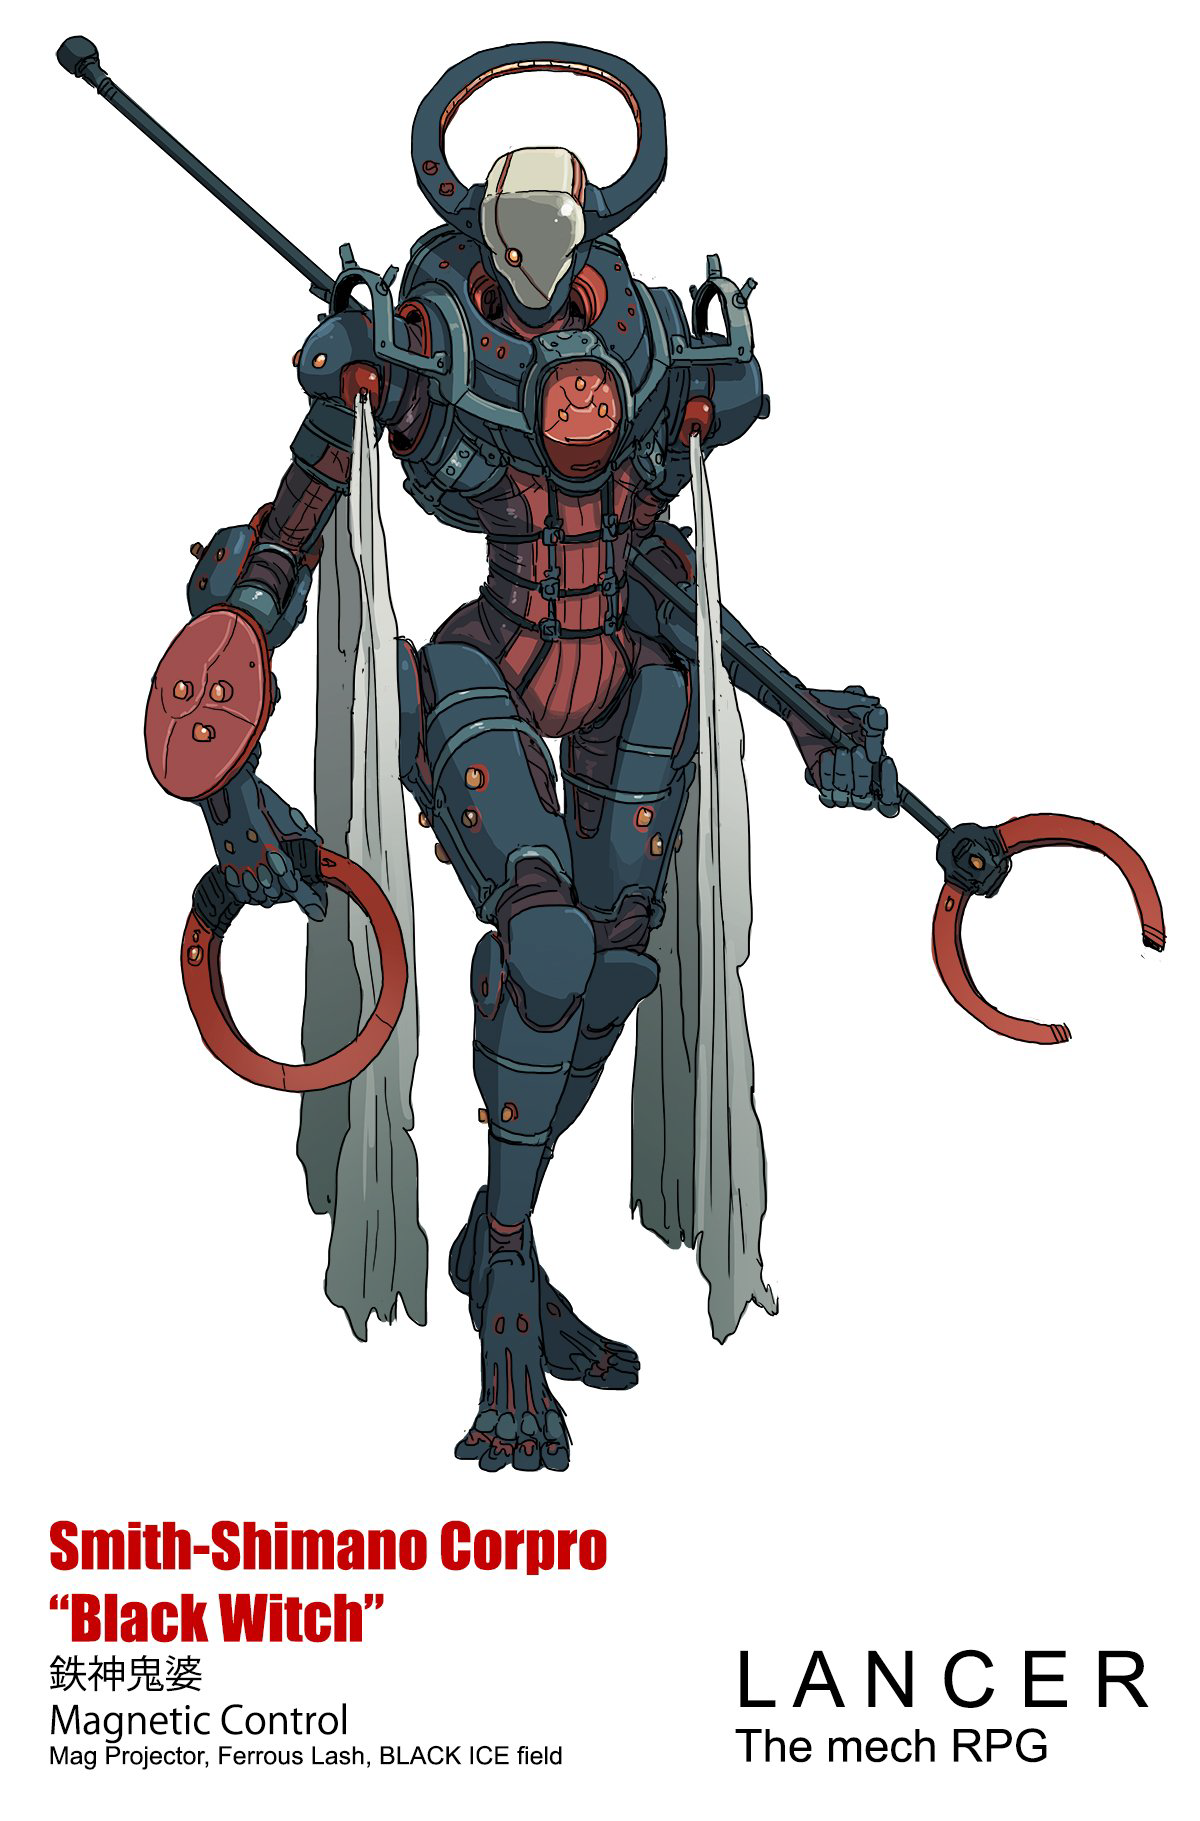
\includegraphics{BlackWitch}
\end{center}

\begin{mech}{SSC}{Black Witch}

\fluff{The BLACK WITCH is the primary designate model in SSC’s newest line of mech cores meant to compete with HORUS’s dominance in the field of invasion/control cores. The BLACK WITCH is open to all pilots with the necessary SSC licensing and should experience greater overall use, as current SSC licenses outnumber the hypothetical maximum of HORUS licenses issued. The BLACK WITCH is built to withstand the stresses of combat system invasion and magnetic weaponry: it is a primary platform for engagements where the use of kinetic, ferrous projectiles and ordinance is expected. Developed primarily as a salvage and scrap repair system, the SSC-BW’s mag field system was soon repurposed by the SSC Gendarme as a personal defense system}

\begin{license}
\item Ferrous Lash, Mag Cannon
\item BLACK WITCH FRAME, ICE-OUT Drone, Mag Deployer
\item Black ICE module, Mag Shield
\end{license}

\frameBox
[hp = 6,
evasion = 10,
speed = 5,
heat cap = 6,
sensors = 15,
armor = 1,
e-defense = 12,
size = 1,
repair cap = 3,
tech attack = +1,
traits = {\textbf{Repulsor field:} The Black witch is resistant to kinetic damage

\textbf{Mag parry:} 1/round you can attempt to parry any attack that deals kinetic damage against you or an adjacent ally as a reaction. Roll a d6. On a 5+, the attack is negated and automatically misses.},
sp = 8,
mount one = aux/aux mount,
mount two = main mount,
core system name = Mag Projector,
core system text = {A magnetic field generator takes the same technology as other projected magnetic defenses and makes them portable separate from a mech core. When activated, the mag field generator creates a projected magnetic bubble that traps all incoming ferrous projectiles; the strength of the field is so great that it can even draw mechs to its center. When the field is canceled or the solid-state battery burns out (by design), the field detonates through sudden catastrophic reversal, launching all captured projectiles out from its center.},
core active name = Mag Field,  
core active text = {As a quick action, you may activate the mag field to create a Blast 4 area in any area with at least one square adjacent to you. Inside, ranged weapon attacks that deal kinetic or explosive damage cannot penetrate into or out of the field and will stop at the edge, doing no damage (keep track of them). The field is difficult terrain for all mechs and vehicles made at least partly of metal. Actors at least partly made of metal that start their turn in the Mag Field or enter it for the first time on their turns must make a successful Engineering check with 1 difficulty or be pulled to the center as far as possible and immobilized. They can repeat this check at the start of their subsequent turns while trapped this way and can move normally on a success, otherwise they remain trapped. The field lasts until the end of your next turn. At the end of your next turn, any kinetic or explosive weapons fired into this field will resume trajectory towards the center of this zone. The GM performs a single attack roll vs each target still inside the zone with +1 targeting per attack fired into this zone (cumulative, up to a max of +6). Successful hits deal 1d6 Kinetic damage per attack fired into this zone (cumulative, to a maximum of 6d6). Then, the zone deactivates.}] 


Mag Cannon

The SSC Magnetic Cannon is a first in Smith-Shimano’s ENERGY line: an aperture-focused magnetic projection beam that disrupts and damages hardware using intense pulses of magnetic force. Cores caught in the beam of a mag cannon suffer additional damage to their software, as even hardened components come under massive systemic stress.

Main Cannon

1 heat (self) 
Line 8 
1d3 energy damage +1 heat

All targets caught in the area of this weapon must pass a systems check or become impaired until the end of their next turn.


Ferrous Lash

Initially developed as a non lethal crowd suppression device, the Ferrous Lash is a far more complex and dangerous device in the right pilot’s hands. Fired from a series of integrated launchers, the FL system detonates payloads of fast-congeal ferrofluids that restrain their targets; tuned to the correct frequency, these proprietary SSC ferrofluid blends form into rudimentary ambulatory segments, pulling their hosts back towards the casting unit. 

2 SP
Quick Action

A target of your choice in range 10 must pass an agility check with 1 difficulty. On a failure, it is knocked back 5 in a direction of your choice. This movement must obey obstructions, terrain, etc, but doesn't provoke reactions and ignores engagement. If it collides with an obstacle or another mech, it is additionally knocked prone. 


ICEOUT drone

SSC’s ICEOUT module is a response to the increasing reliance on system-based scans to ensure accurate targeting. By blanketing a core’s systems in layers of digital defilade, mirroring, spoofing, and redirection, an ICEOUT module can effectively disappear/disincorporate/legion its user from hostile scans. Note that this module only makes its user system-invisible; they will still be visible through optics. 

2 SP, Limited (2)
Drone, quick action

You fire an ICEOUT drone at a point within range 10 of you, where it hovers in place. The drone is invisible. Once fired, the drone creates a burst 2 zone around itself. Any target at least partially covered by the zone, allied or enemy, is immune to all tech actions (even beneficial ones), and cannot make or benefit from any tech actions. Any negative statuses caused by tech actions immediately end. Targets inside the zone don’t show up on any electronic sensors and are only visible to the naked eye or optics. The drone deactivates at the end of the current scene or when destroyed, and cannot be re-used. You can move it again to a point in your sensor range as a quick action.


Mag Deployer
SSC’s own take on flash-printing is advanced enough to embed magtech burnout cells into raw prefab clay. SSC non-mag pilots often disparage Black Witch pilots for “throwing plates” at the enemy, but the tactical advantage they provide cannot be denied. 

2 SP
Quick action.

You flash-print a heavy metal plate that takes up a 2x2 free space in range 5 of you. It is flat and doesn’t obstruct movement. You can set the system to one of two settings when you create it:

         Repulse: Any hostile target that enters the space must pass a hull check or be pushed in a direction of your choice 3 spaces. If this causes them to collide with an obstruction (terrain, a mech, etc) it is additionally knocked prone. An allied target that enters the space can fly 3 in any direction as a free action.

         Attract: Any target, allied or enemy, that enters the space, must pass a hull check or become immobilized. It can end this status by taking a quick action and repeating this check successfully to free itself.

The deployer can be attacked - it has evasion 5, 20 hp, and 2 armor, and it lasts until the end of the current challenge or around an hour outside. You can only deploy one at at time. If you create a new deployer, the old one disintegrates and is destroyed. 


Black Ice module

3 SP, Unique

Hostile tech actions or system attacks against your mech or any adjacent ally are made at +1 Difficulty. Successive attacks in the same combat from any target are made with an additional +1 Difficulty (cumulative). This difficulty has a maximum of +4, and resets when it would hit +5 back to +1 as its definitions roll over.


Mag Shield
SSC’s magnetic shield takes the same technology as their proprietary magnetic buckler and applies it to a massive deployable system.

2 SP, Unique
Shield, quick action

As a quick action, this system creates a line 4 force field 4 spaces high with at least 1 square in an adjacent space to you. Any adjacent mech can use this force field for heavy cover from attacks on the other side. It additionally gains resistance to kinetic and explosive damage from attacks on the other side of this field, but conversely, any of its targets on the other side of the forcefield gain resistance to kinetic and explosive damage from its attacks. The shield lasts until the end of the current scene, but only 1 shield can be placed at a time.
\end{mech}


\section{SSC Death's Head}

\begin{mech}{SSC}{Death's Head}

\fluff{The DEATH’S HEAD is Smith-Shimano’s answer to all other long range, low splash artillery mechs. By sacrificing hull strength for stability and alacrity, the DEATH’S HEAD manages to avoid incoming fire while holding a near-perfect lock through advanced maneuvers.}

\begin{license}
\item Hi Stress Mag Clamps, Tracking Drone
\item DEATH’S HEAD FRAME, Core Siphon, Vulture DMR
\item Kinetic Compensator, Railgun
\end{license}

\frameBox
[hp = 8,
evasion = 10,
speed = 5,
heat cap = 6,
sensors = 10,
armor = 0,
e-defense = 8,
size = 1,
repair cap = 2,
tech attack = +0,
traits = {\textbf{Neuro-linked:} The Death’s Head can re-roll the very first ranged attack it makes per round. It must keep the second result. Perfected Targeting: The Death’s Head gets a bonus +1 to all ranged attacks (a flat +1 to the attack roll)},
sp = 6,
mount one = main/aux mount,
mount two = heavy mount,
core system name = Precognitive Targeting,
core system text = {Precognition is the next step in human/AI interaction. By allowing AI data-dump and REM learning via a neural bridge, a pilot can learn to read situations before they begin to develop. The nature of precognition is as-yet unknown, so SSC recommends limited, monitored use of this protocol.},
core active name = Activate Neural Shunt,
core active text = {For the rest of this scene, you can take the following action:
  Mark for Death
  Full Action
  Choose a target in range 30 but further away from range 5 of the Death’s Head. You concentrate on that target. While concentrating, your mech cannot move or take reactions. You can stop concentrating at the end of any of your turns as a free action, and can only concentrate on one target at once. While concentrating on a target, as long as that target is not in cover from you or within range 5 of you, your ranged attacks against the target deal +4d6 bonus damage on Critical Hit.}]

Hi-stress Mag Clamps

A simple, reliable system. When installed, it seeds toggleable electromagnets into the locomotive systems of a chassis. When turned on, the mag clamps allow a chassis to cling to ferrous surfaces. Of especial use in micro and null gravity environments.

1 SP, Unique

Your mech treats all vertical and overhanging surfaces as flat ground for the purposes of movement. You no longer count as climbing on these surfaces and can move, stand, and run at full speed, though if you are knocked prone you fall.


Tracking Drone

A modified version of a tracer round, a tracking drone must hit its target in order to activate. Once a successful hit is registered, a tracking drone will feed live, surreptitious data back to its shooter across multiple theaters.

1 SP

Quick Tech

Gain the following quick tech action:

Tracking Drone: Make a tech attack against a target in your sensor range. On a hit, you know the target’s exact location, HP, Structure, Heat, and speed, and it cannot hide or benefit from invisibility from you until the drone is removed from them. It takes a quick action and a successful engineering check from the targeted mech to remove a tracking drone.


Core Siphon

By shunting some core waste-heat from dispersal systems to weapon systems, the Death’s Head can overclock its weapons’ targeting, catalytic, and processing systems. This comes with a trade-off, however, as reliance on overclocking without sufficient cooling can damage systems not built to handle the influx of power.

2 SP
Unique

At the beginning of your turn, you can choose to give the first attack roll of your turn +1 Accuracy. If you do, however, any additional attack rolls until the end of your turn gain +1 difficulty


Vulture DMR

The SSC VULTURE-BR is Smith-Shimano’s core line battle rifle, chambered for 12.7x108mm HTI rounds. Field performance reports of the VULTURE report low TTK rates and satisfactory all-theater capability, though some pilots have reported fouled-fire incidents as a result of the high burst rate.

Main Rifle
2 heat (self)
Overcharged, Accurate
Range 15, 1d6+1 kinetic damage


Kinetic Compensator

Another common modification, a system of electronically modulated gyroscopes and hydraulic compensators work in concert to absorb and disperse recoil caused by firing heavy weaponry.

2 SP, Unique

When you miss with any ranged weapon attack roll, your very next ranged attack roll gains +1 Accuracy.


Railgun
A railgun is a simple, elegant weapon. With no moving parts and a magnetically-accelerated projectile, a railgun can be used at peak efficacy in any combat theater and is entirely self- contained in a disposable unit. However, power draw is massive, and it is necessary for mechs mounting a railgun to be fitted with a core-charged auxiliary power pack.

Heavy Rifle
AP, Ordnance
Line 20
1d6+4 kinetic damage

\end{mech}

% \subsection{SSC Dusk Wing}

\begin{mech}{SSC}{Dusk Wing}

\fluff{The SSC DUSK WING is built from a legacy-inspired modification package to hazardous/hardened EVA suits; in the early days of deep space exploration, there was a need for mechanized exoskeletons that provided not only amplified capacity, but plated kinetic defense. The DUSK WING is the spiritual heir of those early deep space suits. Fast and small, the DUSK WING mounts a complement of all-theater maneuverability jets that allow for perfect (or near-perfect) flight.}

\begin{license}
\item Veil Rifle, SSC neurospike Mk1
\item DUSK WING FRAME, Burst Launcher, Flicker Field
\item StunCrown, OASIS
\end{license}

\frameBox
[hp = 6,
evasion = 12,
speed = 7,
heat cap = 5,
sensors = 10,
armor = 0,
e-defense = 8,
size = 1/2,
repair cap = 2,
tech attack = +1,
traits = {\textbf{Integrated Hover Flight:} The Dusk Wing can hover when it moves or boosts (it can fly, doesn't need to move, it can move without going in a straight line, and doesn't need to land). While flying, it generates 1 heat at the end of its turn.

\textbf{Harlequin Cloak:} The Dusk wing is invisible during its turn. It re-appears at the end of its turn.

\textbf{Fragile:} This mech has +1 Difficulty on Hull Checks},
sp = 6,
mount one = aux/aux mount,
mount two = flex mount,
% core system name = -,
% core system text = {-},
core active name = Hall of Mirrors,
core active text = { Active (requires 1 core power): For the rest of the scene, gain the following quick action:
Hall of Mirrors
Each time your mech takes the boost action or its regular move on its turn, it leaves a holographic imprint of itself behind in the space where it started. This hologram is an illusory projected object the same size as your mech (it can be moved through and doesn't actually take up any space). The holograms detonate if any non-allied actor moves through or adjacent to their space, dealing 1d6 energy damage (an actor can pass an agility check to halve this damage). In addition, any time as a quick action, you can instantly teleport to one of the hologram's locations. Doing so detonates all holograms for a burst 1 attack centered on their areas for the same effect and prevents you from generating new holograms until the start of your next turn.}]


Veil Rifle

Main Rifle
Line 10
1d3 energy damage

Allies caught in the area of this rifle do not take damage but are instead are covered in coruscating energy that throws off targeting systems and count as in light cover until the start of your next turn.


SSC Neurospike Mk1

Building off SSC's strain of dormant DHIYED viral code, the Neurospike Mk1 was the first all-theater, single- use spike system developed by the Exotic Materials group. N-Mk1 comes pre-packaged with a basic, but effective, activated DHIYED virus: when fired or otherwise implanted in a synthetic target, it pumps a cocktail of DHIYED virus into the codebase, altering crew outputs and onboard systems' battlefield perception.

2 SP, Unique
Quick Tech

Gain the following options for invasion:

Shrike Code: Until the end of your next turn, each time your target makes an attack roll, it first takes 2 heat.

Mirage: Choose yourself or a friendly mech you can see. Your target's systems relay blurred, illusory images of that mech over its real image that confuse your target's systems. That friendly mech (or your mech) counts as invisible to your target until the end of your next turn.


Burst Launcher

Typically dorsally mounted, Burst Launchers fire rapid streams of explosive cores. These thermal spheres are tuned for an airburst detonation, overwhelming the target zone with rippling chain explosions that damage and suppress units in the area.

Main Launcher
Arcing
Range 10
1d3 explosive damage

On a Critical Hit, a target struck by this weapon is impaired until the start of your next turn.


StunCrown


The SSC StunCrown is a simple system, a ring of WHITEOUT flash lamps in hardened mounts that can be triggered to fire an overwhelming burst of light. The StunCrown is usually mounted on a short post or in a ring around a mech's cranial suite; due to the intense energies running through the flash bulbs, this system only has a limited number of uses before the lights burn out.

2 SP, Limited (2)
Quick action

All hostile targets in a burst 5 area centered on your mech that can see your mech must pass an agility check or become Jammed, and a systems check or become Impaired. Both effects last until the end of your next turn. Mechs in cover from you when this system is activated are not affected.


Flicker Field

Flicker Fields are generated by holochaff, a blend of photoreactive slivers, mirrorchips, LEDs, and strips of flare-out. Fired from launchers at a pilot's command, holochaff looks at first like a cloud of smoke: within moments it adapts to its surroundings and begins to project out a shattered, shifting image of the terrain around it, creating a distorted field that confounds both visual and systemic targeting.

1 SP, Unique

When you move or boost, you project a holographic pattern around your mech that leaves dazzling afterimages, making it hard to discern your mech's location. After moving or boosting you count as having invisibility against the very next attack roll against you. The field disperses after this attack, hit or miss. You can only gain the effect of this field once (you can't `stack' up several instances of it).


OASIS

2 SP, Unique
Protocol
2 heat (self)

Until the start of your next turn when you move or boost you can move only in straight lines, but create a holographic trail behind your mech as you move. The trail lingers until the start of your next turn, creating a light construct 1 space high and the same length as your movement. It can be used for light cover by adjacent allies, and any allies that benefit from this cover also have resistance to energy damage.

\end{mech}


% \subsection{SSC Metalmark}

% \begin{center}
%     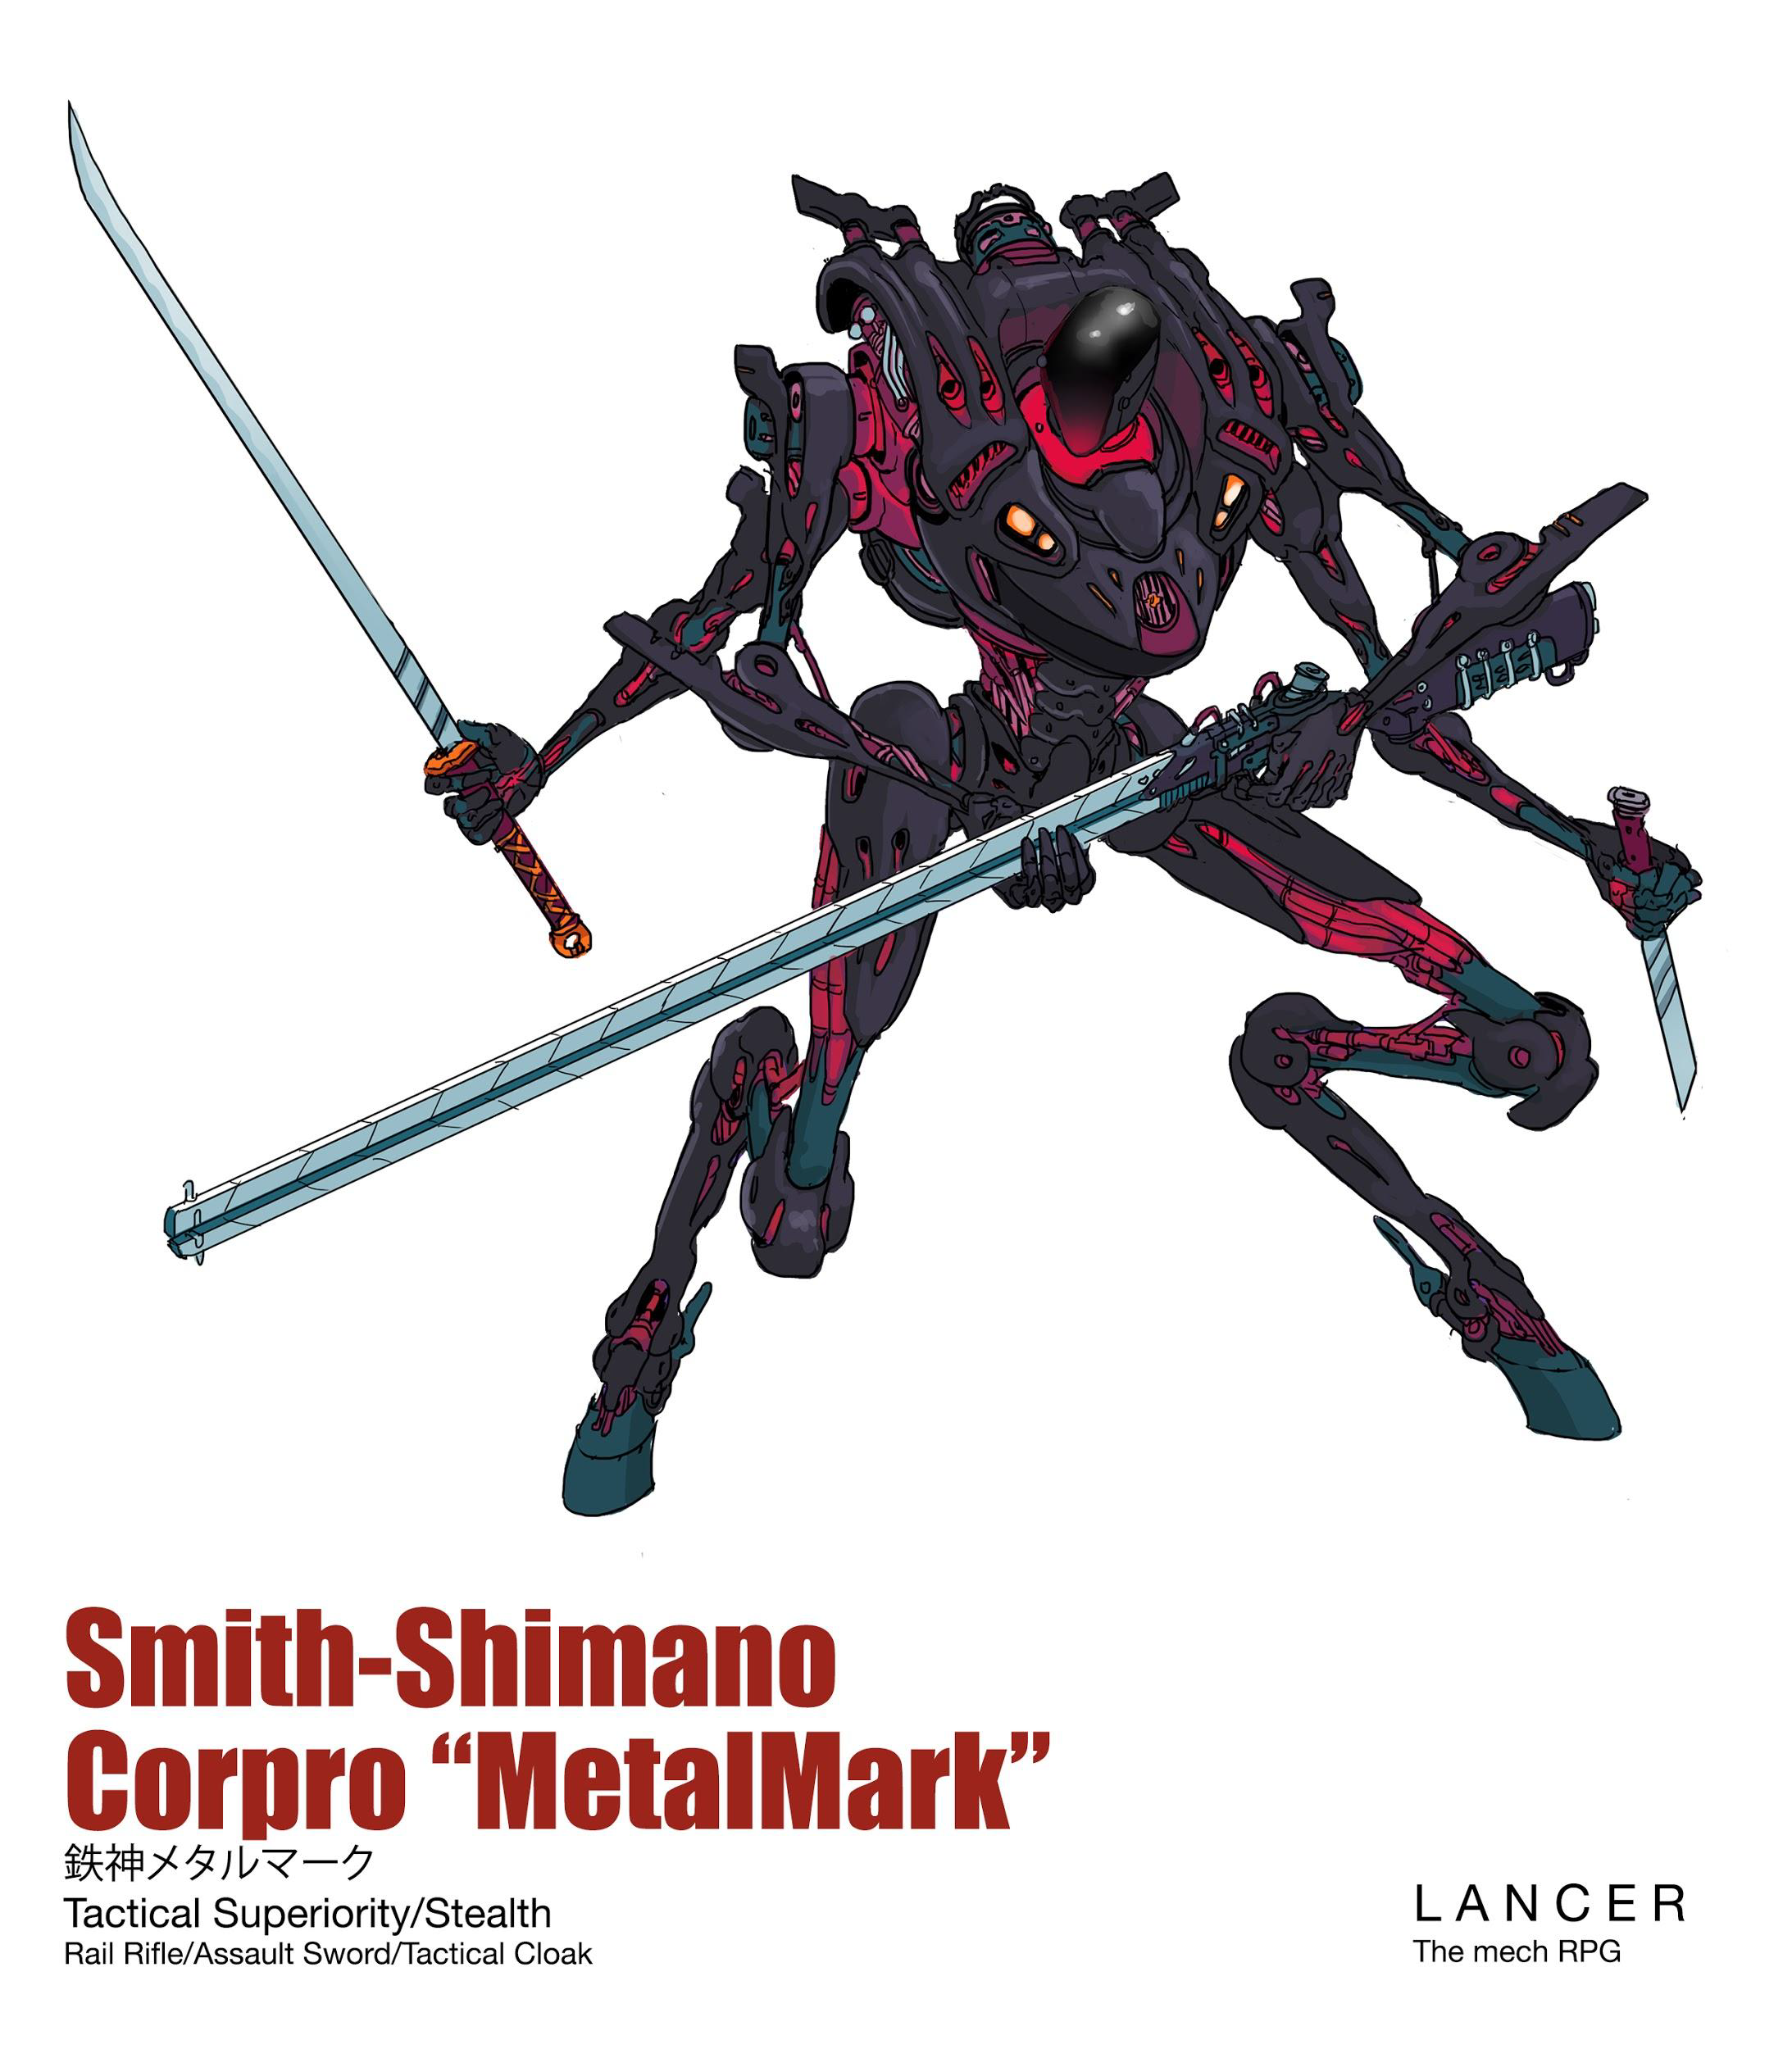
\includegraphics{Metalmark}
% \end{center}

\begin{mech}{SSC}{Metalmark}
\fluff{The METALMARK is SCC's backbone-class line mech, fully equipped with SSC's proprietary design and engineering hallmarks to ensure that it is just as survivable as it is agile. The METALMARK base model reflects SSC's deep-space and long patrol heritage in its aquiline design, sturdy construction, and multiple redundant systems. All METALMARK models come standard with a SMITH CUSTOM LEATHER gimbaled pilot seat to ensure comfort on long distance ranging expeditions.}

\begin{license}
\item Flash Grenade, Reactive Weave
\item METALMARK FRAME, Shock Wreath, Rail Rifle
\item Active Camo, Shock Knife
\end{license}

\frameBox
[hp = 8,
evasion = 9,
speed = 5,
heat cap = 5,
sensors = 10,
armor = 1,
e-defense = 8,
size = 1,
repair cap = 4,
tech attack = +0,
traits = {\textbf{Flash Cloak:} The metalmark is invisible while moving (regular move, boosting, moves from talents, etc), but reappears after it finishes its movement.

\textbf{Carapace Adaptation:} When the METALMARK would benefit from light cover, it instead benefits from heavy cover},
sp = 5,
mount one = aux/aux mount,
mount two = main mount,
mount three = heavy mount,
core system name = Tactical Cloak,
core system text = {A tight-knit, tight-bind weave of reactive fabric, tactical cloaks are high-license tech, restricted to pilots of METALMARK classification II or higher. The weave covers roughly \text{80\%} of a chassis, giving it an overall dull quality when viewed through optics or with the naked eye. It is difficult to target, and when activated it bends light in such a way that makes it nearly impossible to see.},
core active name = Cloaking Protocol,
core active text = {Active (Requires 1 core power):Protocol
Until the end of the current challenge, or when you deactivate this module at the start of your turn, you become invisible. If you take damage, you lose the benefit of this module until the start of your next turn. No other action will deactivate it.}]

\gearBox
[name = {Reactive Weave},
fluff = {A woven CSAJ (Critical Systems And Joints) cover, Reactive Weave not only protects sensitive systems and joints from fouling and poor weather, but provides a surface for SSC engineers to apply their unique loomware technology. This weave is powered, capable of free-flexing to augment a mech's mobility and reduce the stress placed on a chassis' joints.},
template = {1 SP, \Unique},
rules = {When you brace, your mech can immediately move its speed as a reaction and it also gains invisibility until the end of its next turn.}]

\gearBox
[name = {Flash Grenade},
fluff = {},
template = {2 SP, \Limited{2}\newline
\Grenade},
rules = {This grenade can be thrown to a space in range 5. When this grenade explodes, it creates a burst 2 zone that lasts until the end of your next turn. Actors other than you (allied or enemy) caught inside can't trace line of sight out of the zone (they can attack other targets inside normally), and actors inside the zone benefit from light cover.}]

\gearBox
[name = {Shock Wreath},
fluff = {An after-fabrication modification popular among melee-oriented pilots, the Shock Wreath applies an integrated bundle of conductive filaments to the blade, point, tip, or surface of a close combat weapon. Paired with a power source (typically in the hilt or half of a weapon, but sometimes external), the Shock Wreath adds a thermal element to the kinetic, and a distinct visual marker: their weapons are picked out in fine lines of white-hot light, shrouded in heat shimmer.},
template = {2 SP\newline
\Mod},
rules = {Choose 1 melee weapon. It gains Burn depending on its size (Aux: Burn 1, Main: Burn 2, Heavy
or larger: Burn 3). If it already has Burn, this increases the burn it deals by the same amount.}]

\gearBox
[name = {Rail Rifle},
fluff = {A rail rifle is a popular weapon for pilots in any theater, but the only choice for those operating in atmospheres made up of highly combustible gasses. Using a line of cascading electromagnets, a rail rifle accelerates a small projectile up to tremendous speeds, launching it without combustion or heat reactions. A rail weapon is kinetic and comparatively quiet when fired next to combustion weapons, though its energy signature is difficult to mask given the massive power requirements demanded by the weapon system.},
template = {\Main \Rifle\newline
\HeatSelf{1}, \Line{12}\newline
1d6 \kinetic damage}]

\gearBox
[name = {Active Camo},
fluff = {Active camouflage represents the pinnacle of counter-optic defense systems. By interpreting incoming visible-light spectrum data, an active camouflage system can project a light-bending field around its user, effectively hiding them in plain sight.},
template = {3 SP, \Unique\newline
\HeatSelf{2}, \Protocol},
rules = {You can activate or deactivate the light bending properties of this module at the start of your turn. It lasts until the end of your next turn. While this module is active you are invisible. If you take damage, this module immediately deactivates.}]

\gearBox
[name = {Shock Knife},
fluff = {The shock knife is a mech-sized blade made to accept and integrate the post-fabrication Shock Wreathe system. The knives are custom-fabricated by SSC's Terashima artisan enclave, each one bearing its stamp.},
template = {\Auxiliary \Melee\newline
\HeatSelf{1}\newline
\Thrown{5}, \Threat{1}\newline
1 \energy damage + \Burn{2}}
rules={}]
\end{mech}


\section{SSC Monarch}

\begin{mech}{SSC}{Monarch}

\fluff{The SSC MONARCH platform is Smith-Shimano’s solution for a fast, self-propelled missile/barrage battery. Able to mount ground-to-ground, ground-to-air, ground-to-space, and all-theater missile tubes and their guidance systems, the MONARCH can be adjusted to deliver any payload at any distance to any target. The MONARCH is commonly deployed in a fire-support role, though field tests of a MICROMONARCH mid/close range system is underway.}

\begin{license}
\item Sharanga missiles, Companion Gun
\item MONARCH FRAME, Stabilizer weapon mod, Gandiva Missiles
\item Pinaka Missiles, TLALOC class NHP
\end{license}

\frameBox
[hp = 8,
evasion = 8,
speed = 5,
heat cap = 6,
sensors = 15,
armor = 1,
e-defense = 8,
size = 2,
repair cap = 3,
tech attack = +0,
traits = {\textbf{Avenger Silos:} Once a round, when you score a Critical Hit with a weapon, a target different to your first target in range 10 and line of sight takes 3 explosive damage (no roll required).
\textbf{Seeking payload:} The monarch’s launcher attacks against targets suffering from Lock On gain the seeking tag}
sp = 5,
mount one = flex mount,
mount two = main mount,
mount three = heavy mount,
core system name = Avenger silos,
core system text = {The SSC 30 High-pen missile system is a FRAME mounted micro missile system capable of tremendous output in combat. The MONARCH is fitted to hold upwards of 60 of these deadly miniaturized warheads at once.},
core active name = Divine Punishment,
core active text = {Active (requires 1 Core Power): Divine Punishment
Full Action
You unload your Avenger Silos. All targets of your choice on the battlefield (or a burst 50 area from your mech) must pass an agility check with 1 difficulty or take 1d6+3 explosive damage, and half on a suc- cessful save. You do not need line of sight to any targets, and the self-guiding missiles can perfectly seek any target as long as they can trace a path. Once used, you cannot benefit from the Avenger Silos trait until you take a full repair.}]


Sharanga Missiles
  
Main Launcher
Range 15
Arcing
3 explosive damage

When you fire this weapon, you can choose one or two targets in range and line of sight, making attack rolls for each.


Companion Gun

2 SP, Unique

Once a round, whenever you score a Critical Hit against a target, this shoulder-mounted gun can calibrate and rapidly fires a projectile that also deals 3 explosive damage to a different target within range 10 and line of sight, no attack required.


Stabilizer weapon mod

A stabilizer modification is a series of modifications to physical mounts and targeting software that ensures weapons will remain level, steady, and angled at max-optimum in order to ensure positive target engagement at range.

2 SP
Mod
Choose 1 launcher or cannon weapon. Increase its base range by 5, but it gains the ordnance tag.


Gandiva Missiles

Gandiva missiles are a reliable mainstay from Smith-Shimano’s EWAR line. Like the Pinaka, the Gandiva platform is equipped with jet-assisted mid-flight repositioning systems, allowing the Gandiva to respond to changing battlefield environments with a high degree of expected successful navigation to its target. Each Gandiva missile platform comes pre-loaded with a hivemind companion/concierge class drone AI, making an equipped system capable of learning from each right-of-launch experience.

Heavy Launcher
Smart, Seeking, Accurate
1 SP
Range 15
1d6+3 energy damage


Pinaka Missiles

Pinaka missiles are massive, two-stage missiles mounted along the spine of a mech core or carried disassembled, to be affixed and launched from a brachial mount.  Pinaka missiles are adapted from ship-to- ship missiles, their second stage intended to be able to re-orient in flight through jet-assisted repositioning.

Superheavy Launcher
Arcing, 2 heat (self)
Range 30, one or two Blast 1 areas*
2d6+1 explosive damage

When this weapon is fired, it chooses one or two Blast 1 areas within range to attack. The areas cannot overlap.


TLALOC class NHP

TLALOC-Class NHP systems provide advanced multi-system targeting and co-pilot functions, taking over subroutine control to ensure persistent lock-on and engagement. With TLALOC installed and operational, a pilot can trust that their back is always covered and every possible advantage will be exploited. TLALOC clones are often stereotyped as a hasty, impetuous NHP. They are well known for having a superiority complex.

3 SP, Unique
AI

Your mech gains the AI property and the TLALOC protocol

TLALOC protocol

Protocol
2 heat (self)

Your mech is capable of rapidly firing and re-targeting your weapons, far faster than you can think. When you activate this protocol, your mech is immobilized until the start of your next turn, but for the same duration, if you miss any weapon attack, you can immediately re-roll the attack as long as you target a different target in range or area of effect (if the attack was blast, line, or cone). You can take this re-roll only once for each attack (if the second attack misses you don’t get to keep making it), and a target already hit by this attack (from a re-roll or otherwise) cannot be targeted again.

\end{mech}


\section{SSC Mourning Cloak}

\begin{center}
    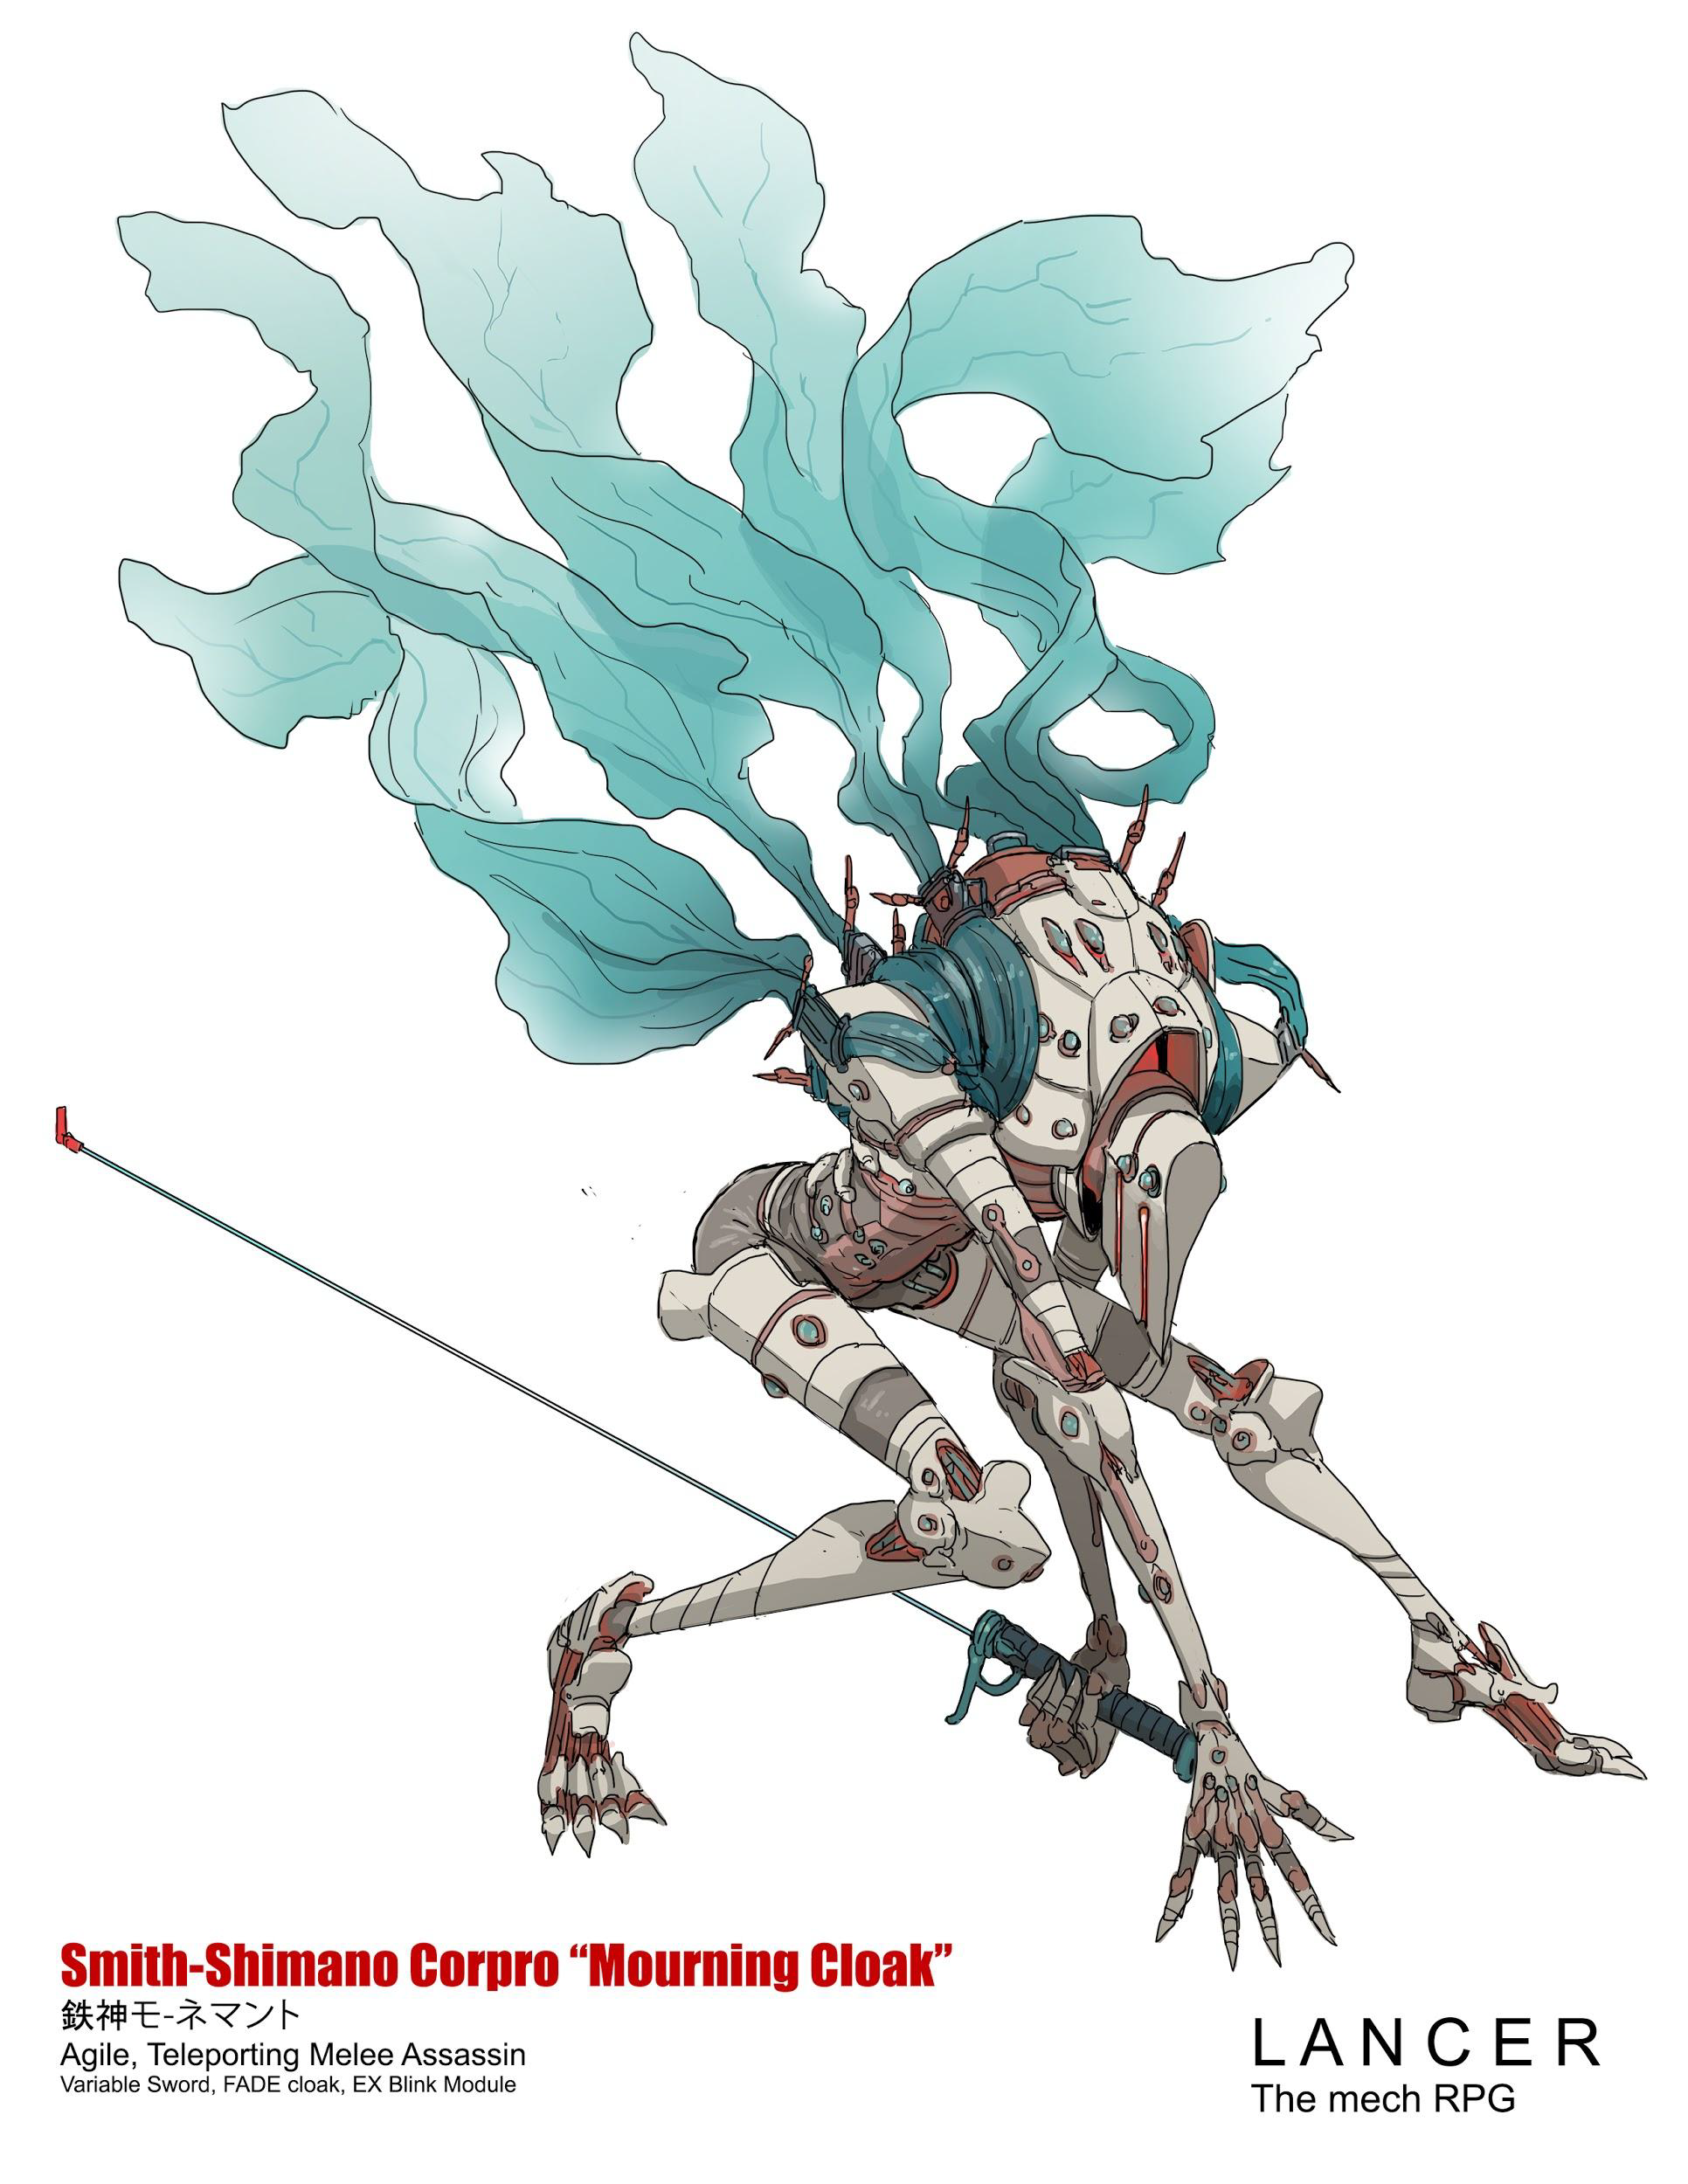
\includegraphics{MourningCloak}
\end{center}

\begin{mech}{SSC}{Mourning Cloak}

\fluff{The SSC MOURNING CLOAK core is intended to provide pilots with a closer-than-CQB tactical option for situations where firearms and ordnance weapons are impractical or unavailable. The MOURNING CLOAK line specializes in precision melee combat and is commonly outfitted with a complement of variable weaponry; shielded microfilament wires designed to attack vulnerable joints and external modules.}

\begin{license}
\item Variable Knife, Vijaya Rockets
\item Mourning Cloak FRAME, Exposed Singularity, Hunter Logic
\item Variable Sword, FADE Cloak
\end{license}
\frameBox
[hp = 8,
evasion = 12,
speed = 5,
heat cap = 4,
sensors = 10,
armor = 0,
e-defense = 6,
size = 1,
repair cap = 3,
tech attack = +1,
traits = {\textbf{Hunter:} The Mourning Cloak’s melee attacks become AP and deal +1d6 bonus damage if it is the only actor (allied or enemy) in engagement with the target

\textbf{Bioplating:} The Mourning Cloak gets +1 accuracy on agility checks},
sp = 6,
mount one = main/aux mount,
mount two = flex mount,
core system name = Smith-Shimano EX Slipstream Module,
core system text = {The EX SLIPSTREAM program is a Smith-Shimano innovation open only to highly licensed pilots. An interesting development in personal travel, the EX SLIPSTREAM module itself is a miniaturized near- lightspeed star drive capable of transporting the user through blinkspace with acceptable accuracy. The program and its technology is temperamental; a mech core is the smallest unit capable of surviving the stress of exposed blink travel, though the experience is still traumatic to the user and those in close proximity to egress.
Passive:
This dangerous and experimental module is a miniaturized starship nearlight drive. You can use it instead of moving or taking the boost action. When you use it, roll 3d6. You can teleport to a point within that range around you as long as there is space for your mech. You don’t have to be able to see this point, but if you attempt to teleport to an already occupied space (by terrain, another mech, etc), the teleport fails and you take 2d6 kinetic damage.
If you roll triples for this system, your mech disappears and does not re-appear, either indefinitely or until your party rests (up to you).},
core active name = Stabilize singularity,
core active text = {Active: Requires 1 core power
Protocol
Until the end of this scene, when you move or boost, you instead teleport up to the same distance.}]


Vijaya Rockets

Vijaya rockets are miniaturized, close range missiles fired from a portable, drum-fed launcher. Their shaped charges are formed in such a way as to project their blast forward, away from the user, and are intended for use in close range engagements as a force multiplier.                                    
   
Auxiliary Launcher

Range 5

Accurate

1d3 explosive damage


Variable Knife

A variable knife is a shorter version of a variable sword, a shielded length of mono-molecular wire. The power drain on a mech’s systems makes mounting these weapons incredible taxing.

Auxiliary Melee

Accurate

Threat 1

2 kinetic damage

The Variable knife deals +1d3 bonus damage on critical hits

Exposed Singularity

SSC’s Exotic Materials project worked to develop the Mourning Cloak’s unique gravatic power plant. For the second generation of the SSC-MC, the Exotic Materials project devised a system that allows pilots to aperture open, for a moment, the gravatic containment system, exposing a slice of naked singularity to realspace. Naked singularity is difficult for organics and synthetics to perceive, being similar to the core of a black hole. The sudden exposure directed at foes (or other targets) essentially “blanks” the Mourning Cloak from real time. The Cloak’s pilot, meanwhile, experiences roughly 10 seconds of normal subjective time, allowing them a brief window in which they can act independently of local realtime. SSC does not recommend abusing this system, as the Exotic Materials group is still testing long-term exposure to local sidereal time.

2 SP, Unique

Reaction

Once per round, when your mech takes damage, you can immediately teleport up to 1d6 spaces as a reaction in a direction of your choosing (though if this teleport would put you inside an obstacle or other mech you take damage as normal and the teleport fails).


Hunter Logic
Building from interpreted strands of DHIYED-strain viral code, SSC’s Hunter Logic is an agile computational memetic, a dual synthetic/VLS-vector systemic weapon capable of crippling a target’s computer and crew.

2 SP


Quick Tech
Gain the following options for invasion:
         - Stalk Prey: Your systems infect the target with a viral logic that wipes your image from their sensors. Until you are damaged by that target, they count you as invisible. This system can only affect one target at a time (other targets still count you as visible and can see you normally).

	        - Terrify: Your systems infect the target with a viral logic that causes your mech to appear horrifying to the target. Until the end of its next turn, your target is impaired and also cannot willingly make any movement that would take it closer to you.


Variable Sword

The variable sword is a Smith-Shimano hallmark. A length of razor sharp molecular wire attached to a handle and caught in a magnetic field, a variable sword is invisible to the naked eye until it makes cuts in an enemy. Built in the early days of interstellar travel, the variable sword was meant to allow for precision sample gathering in the field, while also reducing the overall payload on a mech core.

Main melee

Accurate

Threat 2

3 kinetic damage.

The Variable Sword deals +1d6 bonus kinetic damage on critical hits


FADE Cloak




Representing SSC’s first successful manipulation of what the Aun call the “Firmament”, each Firmament Affinity/Directed Entropy Drive must be fabricated to the unique firmament signatures of the pilot cleared to requisition it. FADE drives are rough tools, artificial affinity generators that allow operators to “shimmer”, to nudge their physical bodies between the causal and paracausal. The drive extrudes a semi-organic membrane that accomplishes this effect, wrapping around the mech. At present, the long-term effects of this system on organic matter is unknown; pilots who are cleared to operate this system agree to check in with their SSC personal concierge on a regular schedule (“check in” includes regular deposits of genetic material).

2 SP
Quick Action, Unique
Once this highly experimental drive is activated as an action, it shifts its user partially in and out of blinkspace. When activated, you immediately go out of phase with reality. While out of phase, you can ignore obstructions such as walls or cover and pass through enemy mechs and solid obstacles as if they were not there, but not end your turn there. You cannot interact with the physical world, but neither can it affect you (in terms of damage, etc). If for any reason you are forced to return while inside of another object, take 2d6 AP kinetic damage and return in the nearest available space.


At the start of each of your turns while this system is active, roll a d6. On a 4+, you go or remain out of phase, on a 3 or lower, you return to the battlefield until the start of your next turn. This drive can’t be activated again if it’s already active. It deactivates if you make an overheating check, deactivate as a quick action, or the scene ends.
\end{mech}

% \subsection{SSC Swallowtail}

% \begin{center}
%     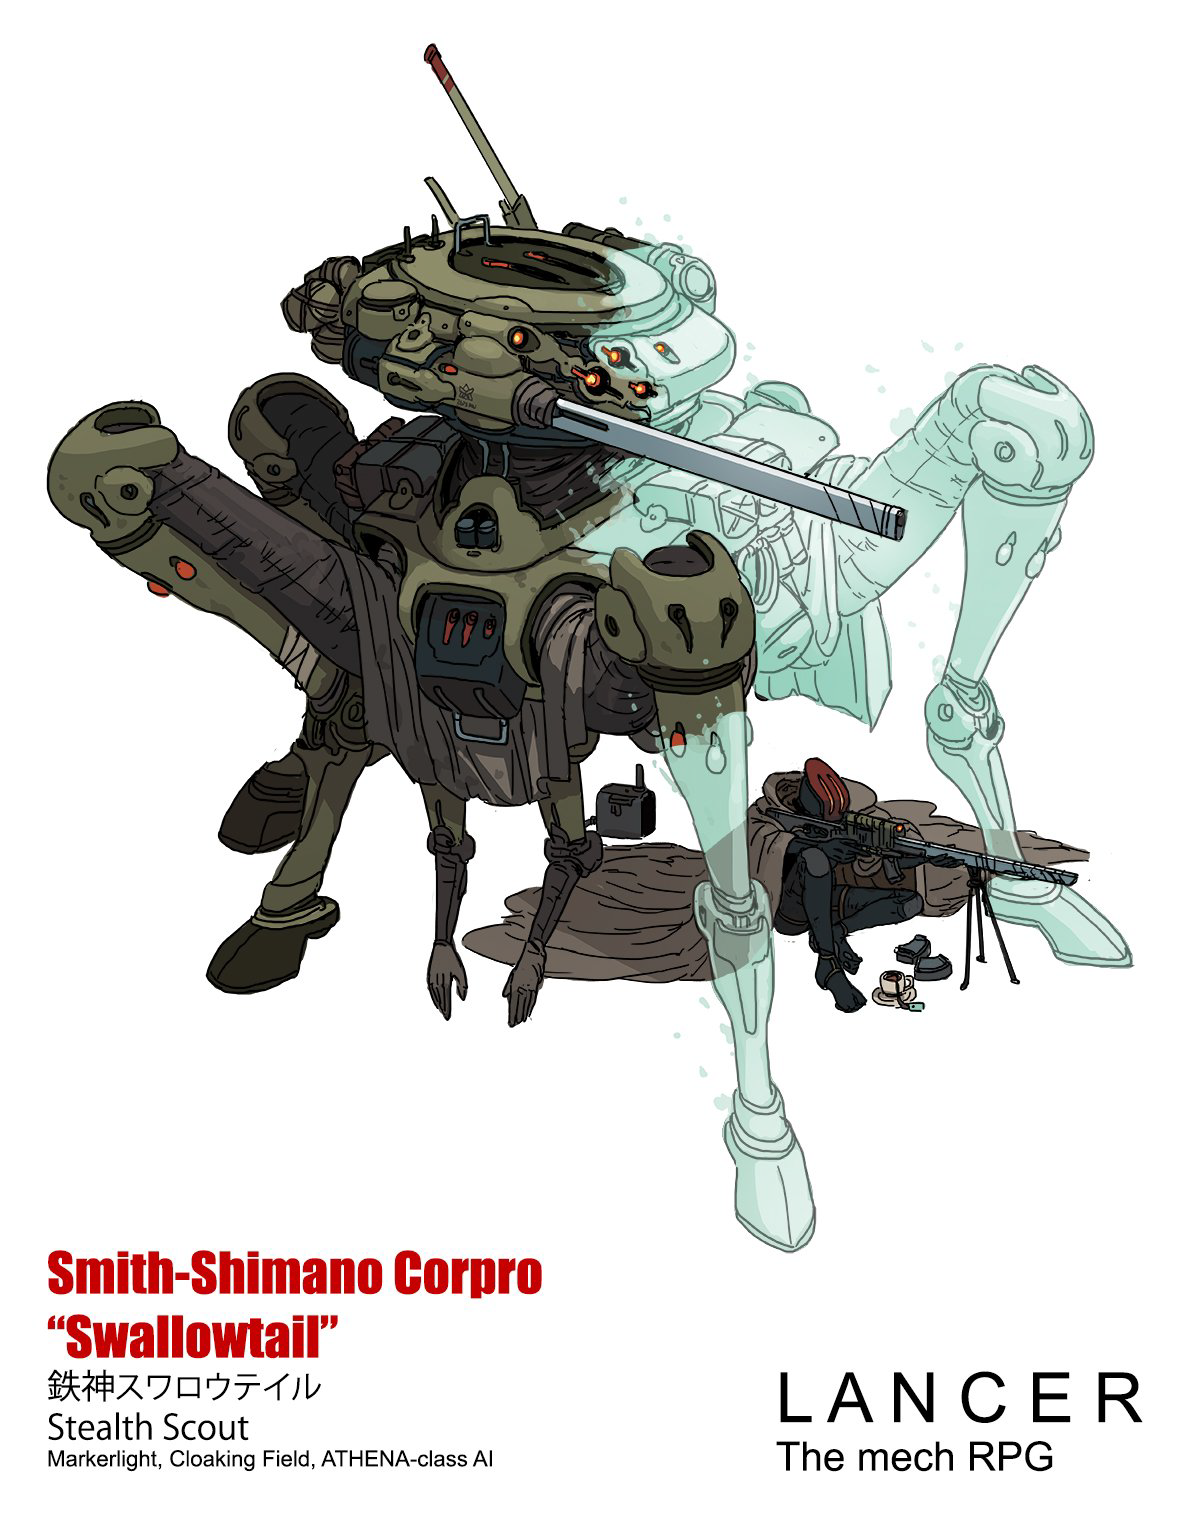
\includegraphics{Swallowtail}
% \end{center}

\begin{mech}{SSC}{Swallowtail}

\fluff{The SWALLOWTAIL platform is Smith-Shimano's primary long range/long term scouting platform, built for rapid and sustained ranging across hostile, volatile environments.}

\begin{license}
\item Markerlight, Scout Drone Nexus
\item SWALLOWTAIL FRAME,  Oracle light machine gun, Low Profile
\item ATHENA-class NHP, Cloaking Field
\end{license}

\frameBox
[hp = 6,
evasion = 10,
speed = 6,
heat cap = 6,
sensors = 20,
armor = 0,
e-defense = 10,
size = 1,
repair cap = 3,
tech attack = +1,
traits = {\textbf{Integrated Cloak:} If the Swallowtail doesn't move during its turn, it becomes invisible at the end of its turn. This invisibility immediately breaks if it moves, attacks, takes a reaction, or starts its next turn.

\textbf{Prophetic Scanners:} Targets suffering from Lock On from the swallowtail are also Shredded},
sp = 6,
mount one = aux/aux mount,
mount two = flex mount,
core system name = Cloudscout TACSIM Swarms,
core system text = {Cloudscout TACSIM Swarms are packets of networked microsensors, launched in nonlethal mortar canisters that detonate high above the battlefield. Once seeded in such a way, the TACSIM program the cloudscouts create begin to run brevity cycles: tight, contained simulations of tactical possibility. Probability results are then fed to the pilot's NHP, who in turn feeds it to the pilot and their networked squad members, ensuring high-probability successful outcomes.},
core active name = Prophetic Interjection,
core active text = {Active (Requires 1 core power):
  Until the end of the current challenge, once per round, as a reaction when an allied target you can see is damaged by another target you can see, you can make a systems check. On success, the attack hitting was actually a simulation that your mech predicted. Your ally gains resistance to all the damage from that attack, and your ally can move 3 in any direction to where they `actually' were. This movement does not provoke reactions and ignores engagement.}]

Scout Drone Nexus

The scout drone is a small, active-camouflaged mini-drone launched from a mounted LOTUS projector. The LOTUS projector fires scout drones at subsonic speeds in bursts of ten, blanketing a wide area with the single-use drones in order to relay information about terrain and targets within.

2 SP
Drone, Quick Action
Sensor Range

When you use this system, you can deploy your drone to an area in sensor range and line of sight. The drone then emits a burst 2 area around it that grants the following benefits:

  - Gain perfect vision of that area

  - Hostile targets that end their turn in the area immediately lose invisibility or hiding.

  - Reveal current HP, Evasion, E-defense, and heat levels of targets in that area

The drone can be attacked and targeted as normal, but it is also permanently invisible. It can be recalled or redeployed by taking this action again.


Markerlight

Main Rifle
1 SP
Range 20

This weapon deals no damage and cannot deal damage (from talents or otherwise) or take weapon mods, but on hit, it inflicts Lock On on your target at the end of your turn.


ORACLE Light machine gun

Auxiliary Rifle
1 SP, Arcing, Accurate
Range 15
1d3 kinetic damage


Low Profile

A hallmark of a well thought out mech platform is the ability for pilots to work with their technicians to adapt their stock model to the specifications of the environments they operate in. Lowering a mech's profile removes extraneous protrusions, tunes any broadcast software, and masks heat signatures — all an effort to reduce optical and scanner signatures.

1 SP, Unique
Protocol

Your mech can retract its major systems to reduce its profile. You can activate this protocol at the start of your turn. While active:

     -   Rolls to find your mech while hidden are made at +1 Difficulty

     -   All ranged and tech attacks against you are made at +1 Difficulty

     -   Your mech is Slowed and cannot make ranged, melee, or tech attacks


ATHENA-class NHP

Smith-Shimano's ATHENA is the pinnacle of total hyperspectral environmental facsimile. Through a combination of unfettered Omninet access, hyperspectral relays fired out from a Cloudscout TACSIM projector, sub-networked squadmates, and active/hostile intrusion protocols, ATHENA bootstraps a near- flawless reconstruction of the immediate environment around its host core. ATHENA is unparalleled in its processing power, and with this reconstructed environment it can provide trustworthy, accurate advising to pilots in need of strategic counsel. ATHENA clones tend to be patient, cautious, and measured in their relations with their pilots.

3 SP, Unique
AI

Your mech gains the AI property and gains the ATHENA protocol:

ATHENA protocol
Quick Action

Choose a blast 3 area within 1 mile of you. Your AI constructs a perfect, real-time, 3d model of this are that you can rotate and interact with, including actors that move in and out of that area, and extreme detail. You can re-target or move this area by taking this quick action again. It lasts until the end of the current scene (or about 10 minutes in narrative time). Your mech gains perfect vision of this area and can relay this to allies, letting any attacks from yourself or allies in the area ignore cover. Hostile targets that end their turn in this area lose invisibility or hiding, and you can see the current heat and HP levels of all targets in the area.


Cloaking Field

SSC's milspec cloaking field is the result of extensive experimentation in cooling and light-reflecting technology. Born from a need to bounce harmful radiation away from ships and EVA modules in deep space, the SSC-MILSPEC LIGHTBEND/OVERCLOAK is a system often equipped by ranger and long-patrol scout pilots to ensure not only radiation protection, but optical concealment as well. The light and radiation-bending properties of the LB/OC conceals anything inside of its projected bubble from sensor suites and optical spotting.

4 SP

2 heat (self)
Quick Action

You can activate or deactivate the light bending properties of this module as a quick action. It lasts until the end your next turn. When you activate this module, your mech and all allied targets within a burst 3 area centered on you become invisible while they remain in the area. This area moves when you move, and remains centered on you. If you become stunned, shut down, or take damage, this module immediately becomes inactive.
\end{mech}
                                                                                                                     

                                                                                                                      


                                                                                                                  

                                                                                                                      

                                                                                                               


                                                                                                                            

                                                                                                                      


                                                                                                             


                                                                                                                        
